\section{Task 2, 3 and 7 - Starting page}
\subsection{The task}
We should have a starting page that shows the user name in the header, the points of the user and a button to play the game.

If an unauthenticated user tries to access the page, he gets redirected to the login page.
\subsection{Main page}
\subsubsection{main.jsp}
This page is just an header for the username, a paragraph for the points and a form with a button to redirect to the game page
\subsubsection{Main.java}
This page is set up at the starting url \textit{\/}, so when the user access the webapp he gets automatically redirected to the login page.

The page itself has only one method, GET, which controls the username saved in the session: if not present, redirects to the login page; if it is the admin, redirects to the admin page (as asked in the task 8); otherwise for a normal user forwards the \textit{main.jsp} page.

We also have a static function to get the user session. This function is used by many pages, and what it does is getting the username and the points from the session; if there is no session or the session does not have an username, it redirects to the login page. In this way we can use just this function to implement the task 7.


\subsubsection{Screenshots}
\begin{figure}[H]
  \centering
  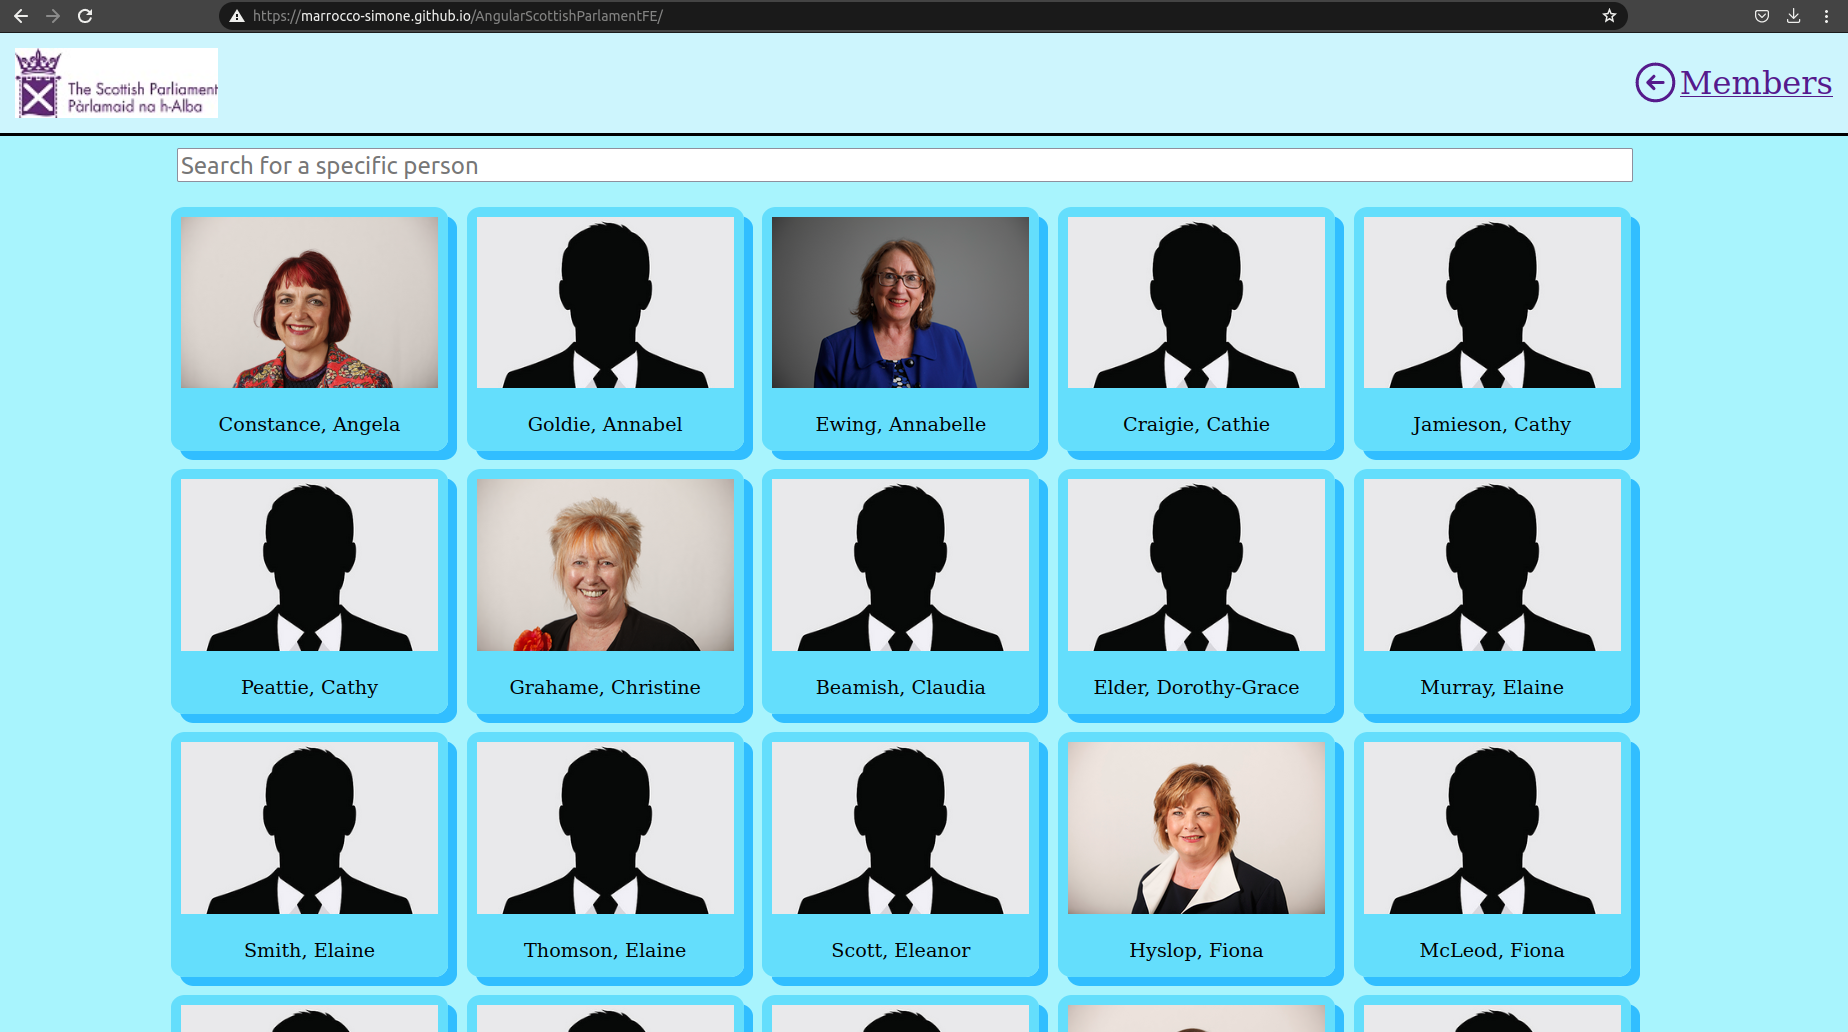
\includegraphics[width=\columnwidth]{main.png}
  \caption{Main Page}
\end{figure}